\documentclass[12pt]{article}

\usepackage{graphicx}
\graphicspath{{../data/}}
\usepackage[a4paper, top=1in, bottom=1in, left=0.8in, right=0.8in]{geometry}

\title{\vspace{-2cm}Is Florida getting warmer?\vspace{-0.5cm}}
\author{\vspace{-0.5cm}Georgina Chow\vspace{-0.5cm}}
\date{\vspace{-0.5cm}November 2024\vspace{-1cm}}

\begin{document}
  \maketitle

  \section{Methods}
  The normality of data for the temperature of different years in Florida was tested using the 
  Shapiro-Wilk test and was found to not reject the null hypothesis (W = 0.98316, p-value = 0.2325).
  Consequently, a Pearson's correlation test was carried out to test whether temperature was correlated
  with year in Florida. To test whether this correlation coefficient value could have been produced by chance,
  randomised sampling of years and temperature values were simulated 1000 times, to obtain sufficient reliabiity 
  of coefficient values.

  \begin{figure}[h!]
    \centering
    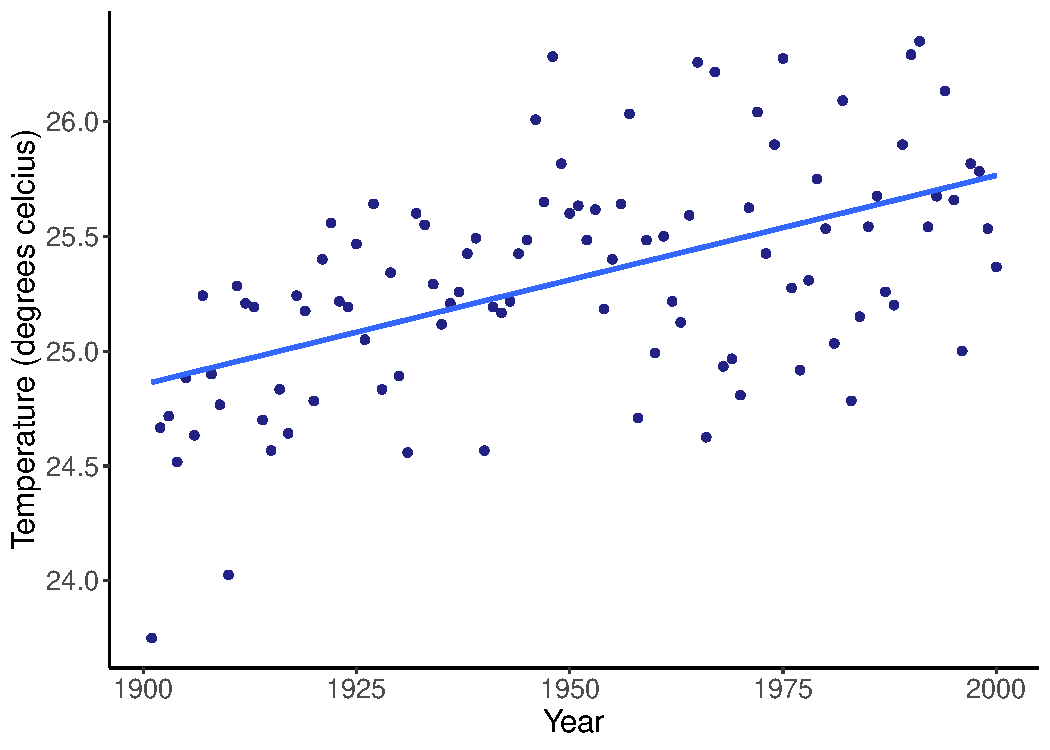
\includegraphics[width=0.8\textwidth, keepaspectratio]{Temp_Year_florida.pdf}    
    \caption{Distribution of average temperatures each year within Florida from 1900 to 2000.}
    \label{fig1}
  \end{figure}

    The observed calculated correlation coefficient (Pearsson) for temperature and year was found to be 
    0.533 (t = 6.24, df = 98, p-value <0.05). Simulation results found that the mean correlation value obtained
    from simulations was 0.0005, with maximum and minimum values ranging from 0.31 to -0.30. Therefore, the 
    asymptotic p-value calculated was found to be 0. 

    \section{Discussion}
    The results from this analysis, looking at the observed and simulation of randomised values, 
    show that the observed correlation between temperature and years in Florida are not obtained by chance 
    and that the null hypothesis should be rejected. There seems to be a moderate positive correlation between 
    temperature and increasing number of years, suggesting that temperatures seem to be rising in Florida.

\end{document}